\section{Reine au tapis}

\lettrine{\jedifont{\$}} Pour les héros du coté lumineux ne peuvent pas laisser un planête entière à la merci de la reine. 

\lettrine{\jedifont{\#}} Les héros du coté obscur y voient une occasion de se faire bien voir du seigneur Vador qui pourra enfin annexer cette planète une fois que la reine sera hors d’état de nuire.

\begin{paperbox}{Objectif}
Tuer la \nameref{sec:ktath-atn-queen}.
\end{paperbox}

Si tout n’est pas clair pour vos joueurs prenez le temps de leur expliquer au travers d’\nameref{sec:aphra}. Les \nameref{sec:symbiote-abersyn}s viennent se loger dans le cortex cérébral et font des victimes des légumes. C’est une sorte de ruche, ils obéissent à la reine et la nourrisse en lui transférant l’énergie vitale de l’hôte. C’est a ça que sert la réception annuelle, la reine est friande de nouvelle énergie, il s’agit de varier le nourriture et de découvrir de nouvelle saveur.

\begin{figure}[h]
\noindent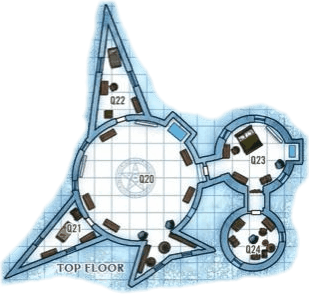
\includegraphics[width=\linewidth]{_img/places/queen-quarter.png}
\caption{appartements de la reine\label{fig:queen-quarter}}
\end{figure}

Une fois que tout est expliqué, ne laissez pas trop les héros cogiter. Les vaisseau qui s’est posé dans la salle de réception a fait un peu de bruit et les \nameref{sec:citadel-guard} ne vont pas tarder a se pointer.
\bigbreak
Les \nameref{fig:queen-quarter} sont accessible, comme les autres niveaux par un escalier mais celui-ci est gardé par deux \nameref{sec:citadel-guard}. Une fois dans les \nameref{fig:queen-quarter}, la reine attendait les héros. Elle a dans ses bras un \nameref{sec:symbiote-abersyn}s qu’elle carresse tendrement, un autre est sur son épaule et un autre en train de lui monter le long de la robe.

\begin{figure}[h]
\noindent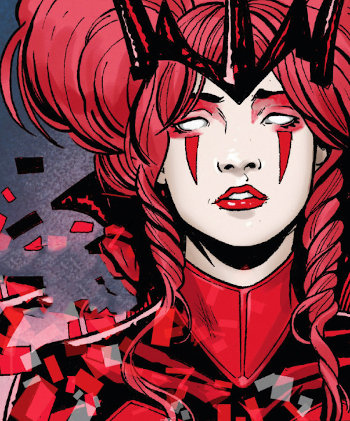
\includegraphics[width=\linewidth]{_img/pnjs/ktath-atn-queen-fight.jpg}
\end{figure}
\begin{quotebox}
\noindent\textbf{\nameref{sec:ktath-atn-queen}}: Finalement, changer de staff n’est pas une mauvaise idée, vous ferez de très bons serviteurs j’en suis sure. C’est moins douloureux si vous vous laissez faire.
\end{quotebox}

La \nameref{sec:ktath-atn-queen} semble vraiment sure d’elle malgrés les héros en sur nombre. Et pour cause, la reine est une magicienne. Il ne s’agit pas de Force mais de techniques anciennes apprise en vampirisant l’énergies de créatures oubliées. Les héros devront faire avec téléportation et chocs psychiques.

Pour les \nameref{sec:symbiote-abersyn}s la manip est la même que pour le combat précédent, chaque tour de jeux un symbiote attaque au hasard un héros.
